\begin{figure}[!htb]
  \centering
  \begin{minipage}{0.5 \textwidth}
    \centering
    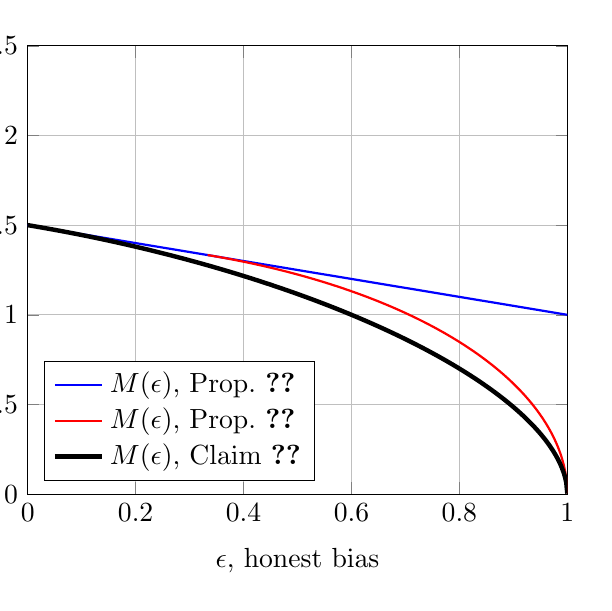
\begin{tikzpicture}[trim axis left,
      declare function={
        entropy(\x) = - \x * ln(\x)/ln(2) - (1 - \x) * ln(1 - \x) / ln(2) ; 
        gamma(\x) = (1 - \x) / 2 + sqrt( 1 - \x^2 ) ; 
        phi(\x) = (3/2) * (1 + \x)^(1/3) * ( 1 - \x )^(2/3) ; 
        }
      ]
      \begin{axis}[domain=0:1,
        samples=500,
        enlarge x limits=false,
        grid=both,
        no markers,
        % there is one default value for the `legend pos' that is outside the axis
        % legend pos=outer north east,
        legend pos=south west,
        % (so the legend looks a bit better)
        legend cell align=left,
        x label style={at={(axis description cs:0.5,-0.1)},anchor=north},
        y label style={at={(axis description cs:-0.1,.5)},anchor=south},
        xlabel={$\epsilon$, honest bias},
        % ylabel={$M(\epsilon)$},
        xmin=0,xmax=1,ymin=0,ymax=2.5
        ]
        \addplot +[thick,blue] {(3 - x)/2};
        \addlegendentry{$M(\epsilon)$, Prop.~\ref{prop:praos-moments-simple}};

        \addplot +[thick,domain=(1/3):1,red] {sqrt(2 * (1 - x^2))};      
        % \addplot +[thick,dotted,domain=(1/1.414):1,red] {sqrt(2 * (1 - x^2))};
        \addlegendentry{$M(\epsilon)$, Prop.~\ref{prop:praos-moments-simple-large-eps}};

        % \addplot +[thick,blue] { ((1-x)/2)^(2/3) * (1 + x)^(1/3) * 2^(entropy(x)) };
        % \addlegendentry{$\MeanRoot$, Prop.~\ref{coro:praos-moments-simple-large-eps}}

        \addplot +[ultra thick,black] plot (\x, { gamma(\x) } );  
        \addlegendentry{$M(\epsilon)$, Claim~\ref{claim:t2star-exact}};
        %\addplot +[thick,black, dotted] { sqrt(2) * (1-x)/2+sqrt(1 - x^2)};  
        %\addplot +[thick,dotted,black] {(3/2)(1+x)^(1/3)(1-x)^(2/3)};  
      \end{axis}
    \end{tikzpicture}
  \end{minipage}%
  \begin{minipage}{0.5 \textwidth}
    \centering
    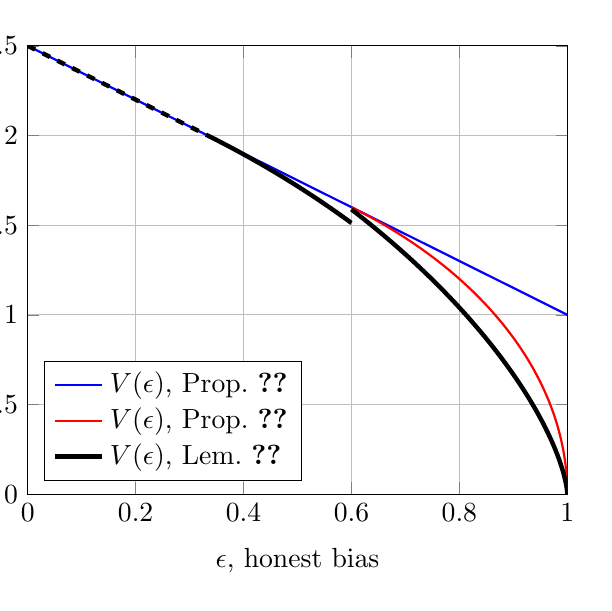
\begin{tikzpicture}[trim axis left,
      declare function={
        entropy(\x) = - \x * ln(\x)/ln(2) - (1 - \x) * ln(1 - \x) / ln(2) ; 
        gamma(\x) = (1 - \x) / 2 + sqrt( 1 - \x^2 ) ; 
        phi(\x) = (3/2) * (1 + \x)^(1/3) * ( 1 - \x )^(2/3) ; 
        psi(\x) = ( 1 - ln( (1+\x)/(1-\x) ) / ln(2) )^2 * ln(2) / 63; 
        }
      ]
      \begin{axis}[domain=0:1,
        samples=500,
        enlarge x limits=false,
        grid=both,
        no markers,
        % there is one default value for the `legend pos' that is outside the axis
        % legend pos=outer north east,
        legend pos=south west,
        % (so the legend looks a bit better)
        legend cell align=left,
        x label style={at={(axis description cs:0.5,-0.1)},anchor=north},
        y label style={at={(axis description cs:-0.1,.5)},anchor=south},
        xlabel={$\epsilon$, honest bias},
        % ylabel={$V(\epsilon)$},
        xmin=0,xmax=1,ymin=0,ymax=2.5
        ]
        \addplot +[thick,blue] {(5 - 3 * x)/2};
        \addlegendentry{$V(\epsilon)$, Prop.~\ref{prop:praos-moments-simple}};

        \addplot +[thick,domain=(3/5):1,red] {2 * sqrt((1 - x^2))};      
        % \addplot +[thick,dotted,domain=(1/1.414):1,red] {sqrt(2 * (1 - x^2))};
        \addlegendentry{$V(\epsilon)$, Prop.~\ref{prop:praos-moments-simple-large-eps}};

        % \addplot +[thick,blue] { ((1-x)/2)^(2/3) * (1 + x)^(1/3) * 2^(entropy(x)) };
        % \addlegendentry{$\MeanRoot$, Prop.~\ref{coro:praos-moments-simple-large-eps}}

        \addplot +[ultra thick,domain=0:(1/3),black,dashed,forget plot] {(5 - 3 * x) / 2};
        \addplot +[ultra  thick,domain=(1/3):0.6,black,forget plot] {2^(2/3) * phi(x)};
        \addplot +[ultra thick,domain=0.6:1,black] { 5/3 * phi(x) )};
        % \addplot +[ultra thick,domain=0.6:1,black] { 2^(2/3 + psi(x) ) * phi(x) )};
        \addlegendentry{$V(\epsilon)$, Lem.~\ref{lemma:grinding-praos-second-moment}};


      \end{axis}
    \end{tikzpicture}    
  \end{minipage}

  \caption{
    Moment (upper) bounds for the grinding power.
    Specifically, let $\epsilon \in (0,1)$ be the honest bias, i.e., $\Pr[\text{a slot is adversarial}] = (1-\epsilon)/2$.
    Let $W$ be a characteristic string of length $n$, $W \sim \mathcal{L}_n((1-\epsilon)/2)$.
    Let $g(W)$ be the grinding power of $W$.
    Suppose $\Exp g(W) = \Poly(n) M(\epsilon)^n$ and $\Exp g(W)^2 = \Poly(n) V(\epsilon)^n$. 
    Above, we have plotted $M(\epsilon)$ (left) and $V(\epsilon)$ (right).
    Note that $M(\epsilon) \leq 1$ for $\epsilon \geq 0.6$, and 
    $V(\epsilon) \leq 1$ for $\epsilon \geq 0.81$. 
    This implies that for those $\epsilon$, the grinding power $g(W)$ is actually $\Poly(n)$.
    % $n$ nonce-generating slots with $\Pr[\text{slot adversarial}] = (1 - \epsilon)/2$, i.e., 
    % The black curve is the asymptotic bound from Claim~\ref{claim:t2star-exact}.
  }
  \label{fig:praos-gp-moments}
\end{figure}
